\section{Evaluation}
\autoref{sub:ts-vast} and \autoref{sub:ts-pub} show how TimeSets can support making sense of complex temporal relationships in intelligence and publication analysis, respectively. In this section, we formally evaluate the performance of TimeSets in lower level and more concrete tasks.

\subsection{Method}
We conducted a lab controlled experiment to compare task performance between TimeSets and a state-of-the-art visualization technique. However, as discussed in \autoref{sub:ts-review}, to the best of our knowledge, no existing techniques are designed to show both multiple-set relations and temporal information of events simultaneously. Therefore, rather than evaluating both the layout and the set visualization technique of TimeSets, we decided to focus only on the second contribution. We compared TimeSets with a set visualization technique that can be applied on top of an existing timeline. We chose KelpFusion~\cite{Meulemans2013} because among similar techniques, it has been shown to have the best performance in readability tasks, regarding both accuracy and completion time. We acknowledged that KelpFusion was not specifically designed to work with timelines. However, KelpFusion can work with any given layouts, and it is the best choice for this evaluation. Our experiment followed a within-subject design; accuracy, time and user preference were collected.

\subsubsection{Datasets}
We used generated data for the experiment to avoid that participants might be distracted from their prior knowledge. Only time-point events were used because KelpFusion can only take input as a set of points. The complexity of the dataset was controlled by two parameters: the number of sets and the average number of events per set. Overall, half of the events were multiple-set, the same ratio as in a real-world dataset used in \autoref{fig:ts-overview}. The details of the four levels of complexity used in the experiment are shown in \autoref{table:dataset}.

\begin{table}[!htb]
\centering
\sffamily\small
\caption{Dataset Statistics.}
\label{table:dataset}
\begin{tabular}{cccc}
	\toprule
	\textbf{Complexity} & \textbf{\# Sets} & \textbf{\# Events} & \textbf{\# Intersections} \\
	\midrule
	Level 1 & 3 & 30 & 15 \\
	Level 2 & 3 & 45 & 23 \\
	Level 3 & 5 & 50 & 25 \\
	Level 4 & 5 & 75 & 38 \\
	\bottomrule
\end{tabular}
\end{table}

%We introduce four approaches to visualize intersections between more than two sets; however, evaluating all of them would triple the number of trials and make the experiment too long. We plan a separate experiment to study which method is the most effective as our future work. In this experiment, we only tested two-sets intersections and simple white circles are used for events' time indicators.

Images of these datasets using the KelpFusion method were generously provided by the method's author. To avoid bias, our method also used static images instead of interactive visualizations. Colors for both methods were Qualitative Set 2 of ColorBrewer~\cite{Harrower2003}. KelpFusion does not have its own layout; therefore, our layout algorithm was used for both settings. Only one algorithm was used to prevent adding another factor to the experiment, which doubles the number of trials for participants. The traceability algorithm was chosen because reading comprehension is not required for the tasks. \autoref{fig:ts-evaluation} shows example images used in the experiment.

\begin{figure}[p]
	\centering
	\subcaptionbox{TimeSets.\label{fig:ts-evaluation1}}{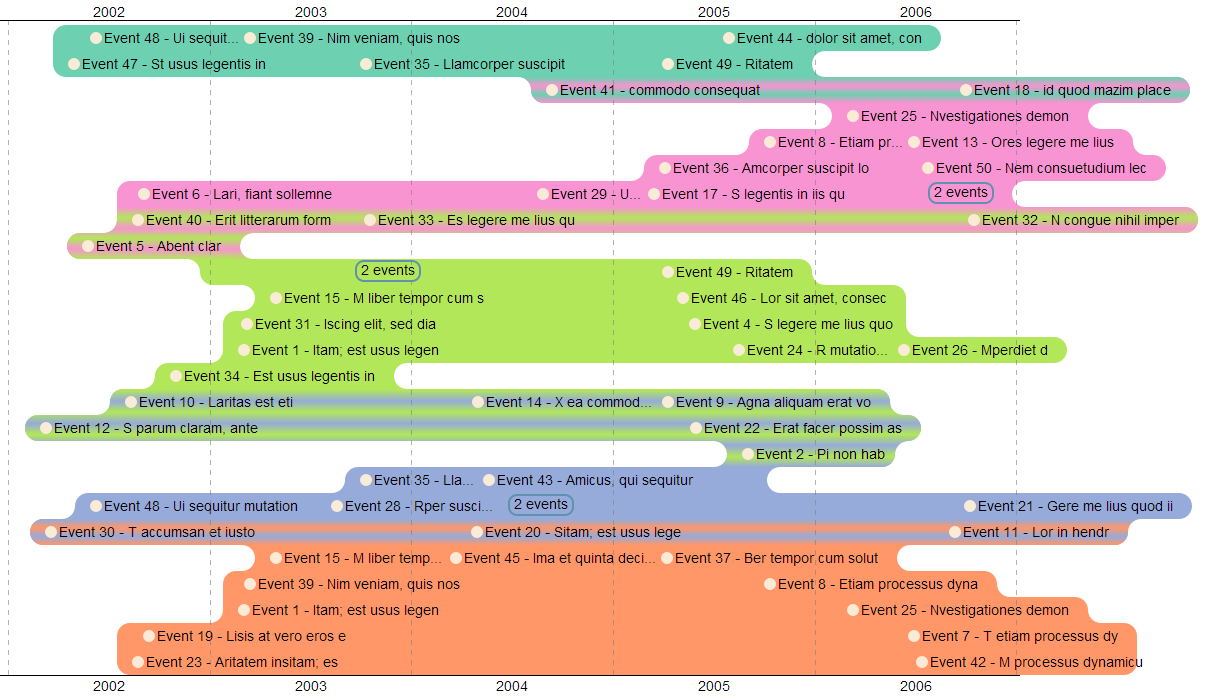
\includegraphics[width=\linewidth]{figure14a}}\\
	\subcaptionbox{KelpFusion.\label{fig:ts-evaluation2}}{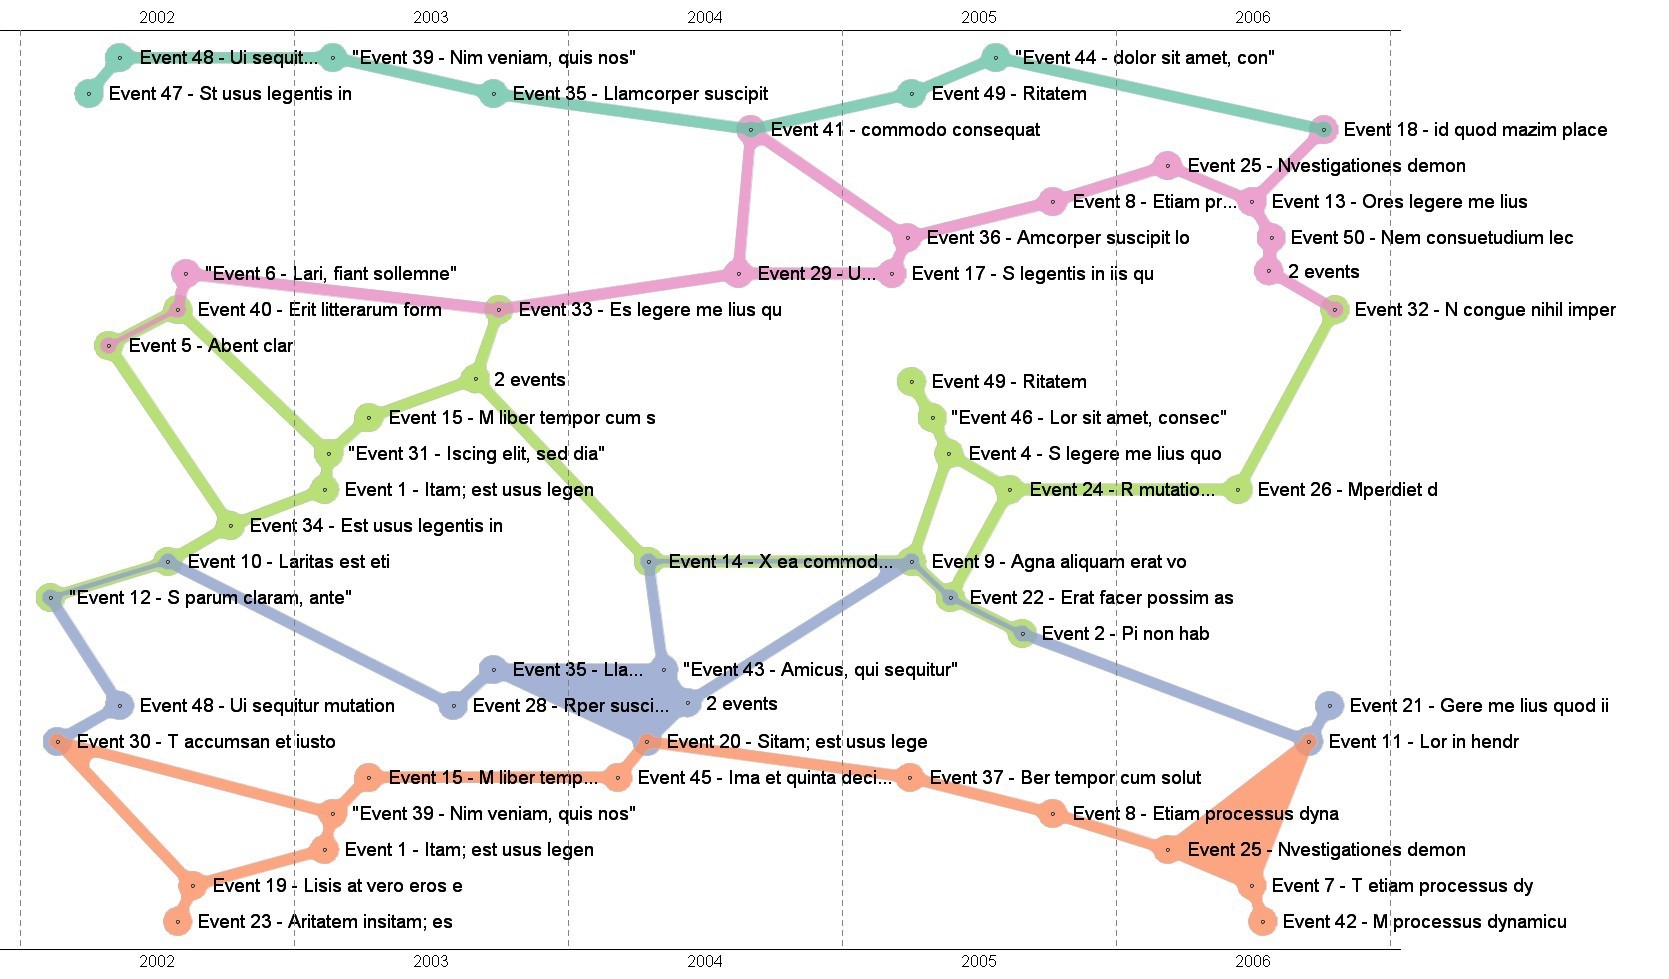
\includegraphics[width=\linewidth]{figure14b}}
	\caption{Example images used in the experiment.}
	\label{fig:ts-evaluation}
\end{figure}

\subsubsection{Tasks} We followed the task design in the evaluation of KelpFusion~\cite{Meulemans2013}, including tasks for estimation and precise comparison of set sizes, and counting the number of elements in a set. Two time-related tasks were added to evaluate the temporal aspect of the  visualization, resulting five tasks in total. Three categories of set readability tasks are considered including the \textit{set} itself, the \textit{intersection} of two sets, and the \textit{difference} between two sets. However, it was impractical to include all 5 $\times$ 3 task types in the experiment. Therefore, we decided to use a combination of them: two tasks for the set itself, two tasks for the intersection, and one task for the difference. All tasks together with examples are listed in \autoref{table:tasks}. Each participant would complete a total of 40 questions.

\begin{table}[!htb]
\centering
\sffamily\small
\caption{Tasks used in the experiment.}
\label{table:tasks}
\begin{tabular}{rl}
	\toprule
	\textbf{Task} & \textbf{Example} \\
	\midrule
	SetOverview & Roughly estimate which set has more events:  A or B \\&(please do \textbf{NOT} count the number of events)? \\
 	IntersectionCompare & Which set pair shares more events: A\&B or C\&D\\&  (please count the number of events)? \\
 	DifferenceCount & How many events are there that belong to the set A \\&but not its neighboring sets? \\
 	SetBiggestYear & In which year does set A have the most events? \\
 	IntersectionPattern & During 2002--2004, what is the change pattern in the \\& number of  events shared by set A\&B?\\
	\bottomrule
\end{tabular}
\end{table}


We used general questions to preserve the external validity of the experiment. It is straightforward to convert them into context-sensitive questions. For example, in the context of \textit{news media}, the last task can be transformed to ``What is the trend of news articles related to both science and fashion during the last 3 years?''. We chose to use multiple-choice answers to reduce the completion time, allowing the within-subject comparison to finish within a reasonable time. This reduces the possible effect of boredom or fatigue as confounding factors. It also avoids considering the typing speed of subjects while evaluating time taken to complete tasks.

\subsubsection{Participants and Apparatus} Thirty students (23 males, 7 females) voluntarily participated in the experiment. They came from various backgrounds including computing, law and psychology. One participant was under 19, 16 participants were aged between 19--25, 12 were aged between 26--39, and one was aged between 40--60. All participants reported that they can distinguish all colors used in the experiment. They completed the experiment using a 23-inch monitor with a resolution of 1920 $\times$ 1080.

\subsubsection{Procedure} The study lasted approximately 45 minutes and consisted of two sessions (one for each visualization technique), followed by a questionnaire. At the beginning of each session, the visualization technique was explained, and participants were shown how to answer each question type using that method. This was followed by five practice questions to familiarize participants with the tasks and the experiment interface. Solutions and explanations were given for these practice questions to help them gain better understanding.

We used two question sets with comparable difficulty and counterbalanced the order of the visualization techniques as well as the order of question sets to reduce learning effects. We fixed the order of task types and the order of difficulty in each type from simple to complex. For each task, the question and all answer options were displayed without the visualization first. Once participants finished reading, they clicked on a button to reveal the figure, and the timing started. This is to reduce the affect of individual differences in reading speed on the measured time.

\subsection{Hypotheses}

For task performance, we hypothesized that
\begin{description}
	\item [H1.] Overall, TimeSets will outperform KelpFusion in both time and accuracy. The colored backgrounds of sets in TimeSets produce a stronger sense of grouping than the connected paths in KelpFusion. Also, in TimeSets, shared events are visually connected, separated from the non-shared ones.

	\item [H2.] For the \emph{SetOverview} task, participants using TimeSets will be faster but less accurate than using KelpFusion. In TimeSets, the colored background makes sets more noticeable; however, the colored area is not always proportional to the set size, which may lead to a misunderstanding for participants.

	\item [H3.] For both the \emph{IntersectionCompare} and \emph{IntersectionPattern} tasks, TimeSets will outperform KelpFusion in both time and accuracy. In TimeSets, shared events are visually connected in its own layer, whereas in KelpFusion, they are mixed with non-shared events.

	\item [H4.] For the \emph{DifferenceCount} task, TimeSets will outperform KelpFusion in both time and accuracy. In TimeSets, events that do not belong to neighboring sets have their own layer with a unique background color, whereas in KelpFusion, they are mixed with the shared events.

	\item [H5.] For the \emph{SetBiggestYear} task, KelpFusion will outperform TimeSets in both time and accuracy. When focusing on events in each year, connected lines in KelpFusion make it easier to count.
\end{description}

For user preference, we hypothesized that
\begin{description}
	\item [H6.] Participants will be more confident with TimeSets because it provides better visual support, especially in intersection and difference tasks.

	\item [H7.] TimeSets will be more aesthetically pleasing than KelpFusion with smooth curves and smooth color changes compared to straight lines and plain colors.

	\item [H8.] TimeSets will be less cluttered than KelpFusion because it uses simple shapes, whereas KelpFusion uses a combination of lines and areas.

	\item [H9.] TimeSets will provide a stronger sense of grouping than KelpFusion because it colors the entire background of a set.
\end{description}

\subsection{Results}
We used a repeated-measure analysis of variance (RM-ANOVA) to analyze the task accuracy and completion time. Accuracy is measured as the percentage of correct answers, and the logarithm of completion time is used to normalize its skewed distribution.

\subsubsection{Accuracy}
\autoref{fig:accuracy} shows the mean accuracy. The RM-ANOVA test revealed a significant main effect of visualization technique ($F(1,29)=4.99, p<.05$), showing that accuracy was significantly higher with TimeSets. There was also a significant main effect of task type ($F(4,116)=8.89, p<.00001$). No significant effect of the visualization $\times$ task interaction was found ($F(4,116)=1.85, p=.12$). Paired t-tests were conducted to investigate the performance difference for each task. A significant effect was found in three tasks: IntersectionCompare ($p<.05$), DifferenceCount ($p<.01$), and IntersectionPattern ($p<.05$), indicating TimeSets was significantly more accurate than KelpFusion in them. Only the task DifferenceCount still had a significant effect with corrected p-value for multiple tests using Bonferroni correction.

\begin{figure}
	\centering
	 {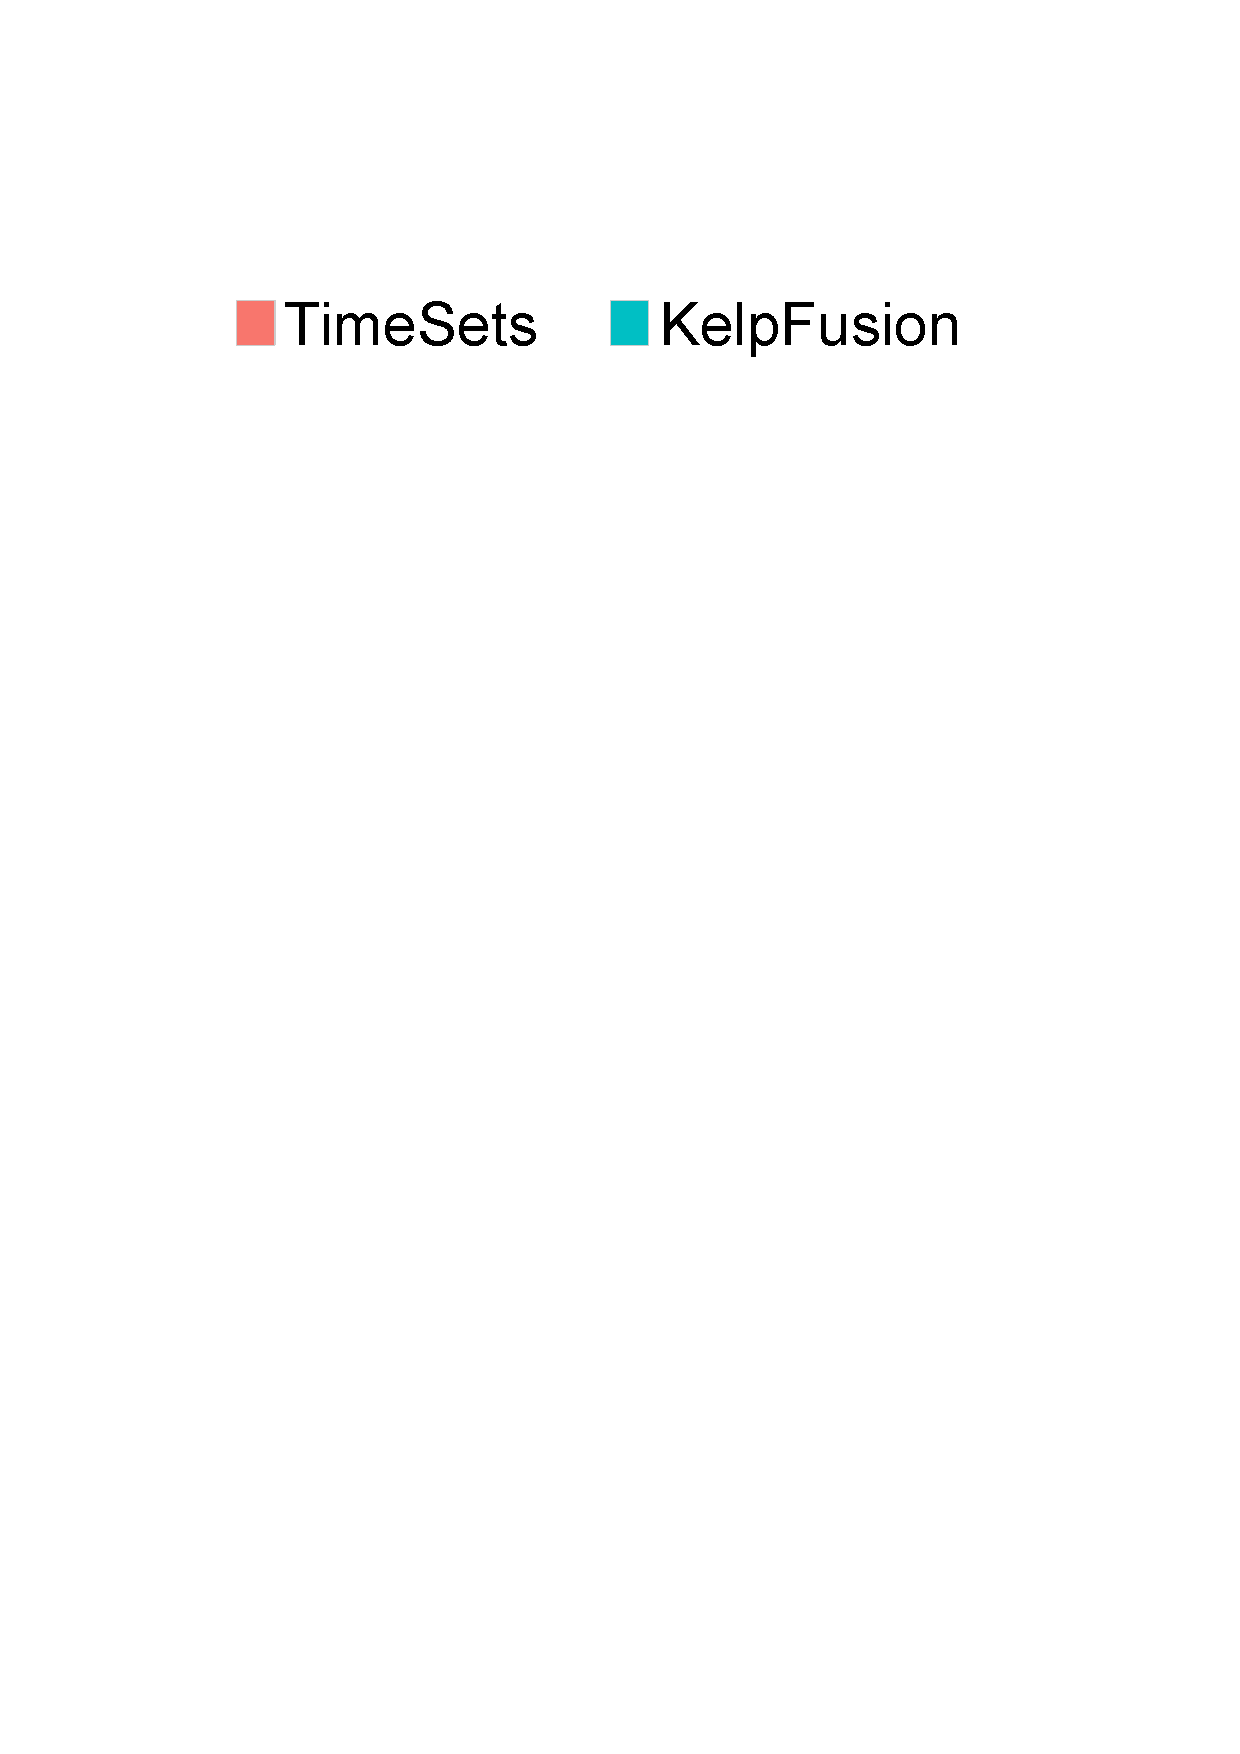
\includegraphics[width=.4\linewidth]{figure15a}} \\
	\subcaptionbox{Mean accuracy (in percentage).\label{fig:accuracy}}{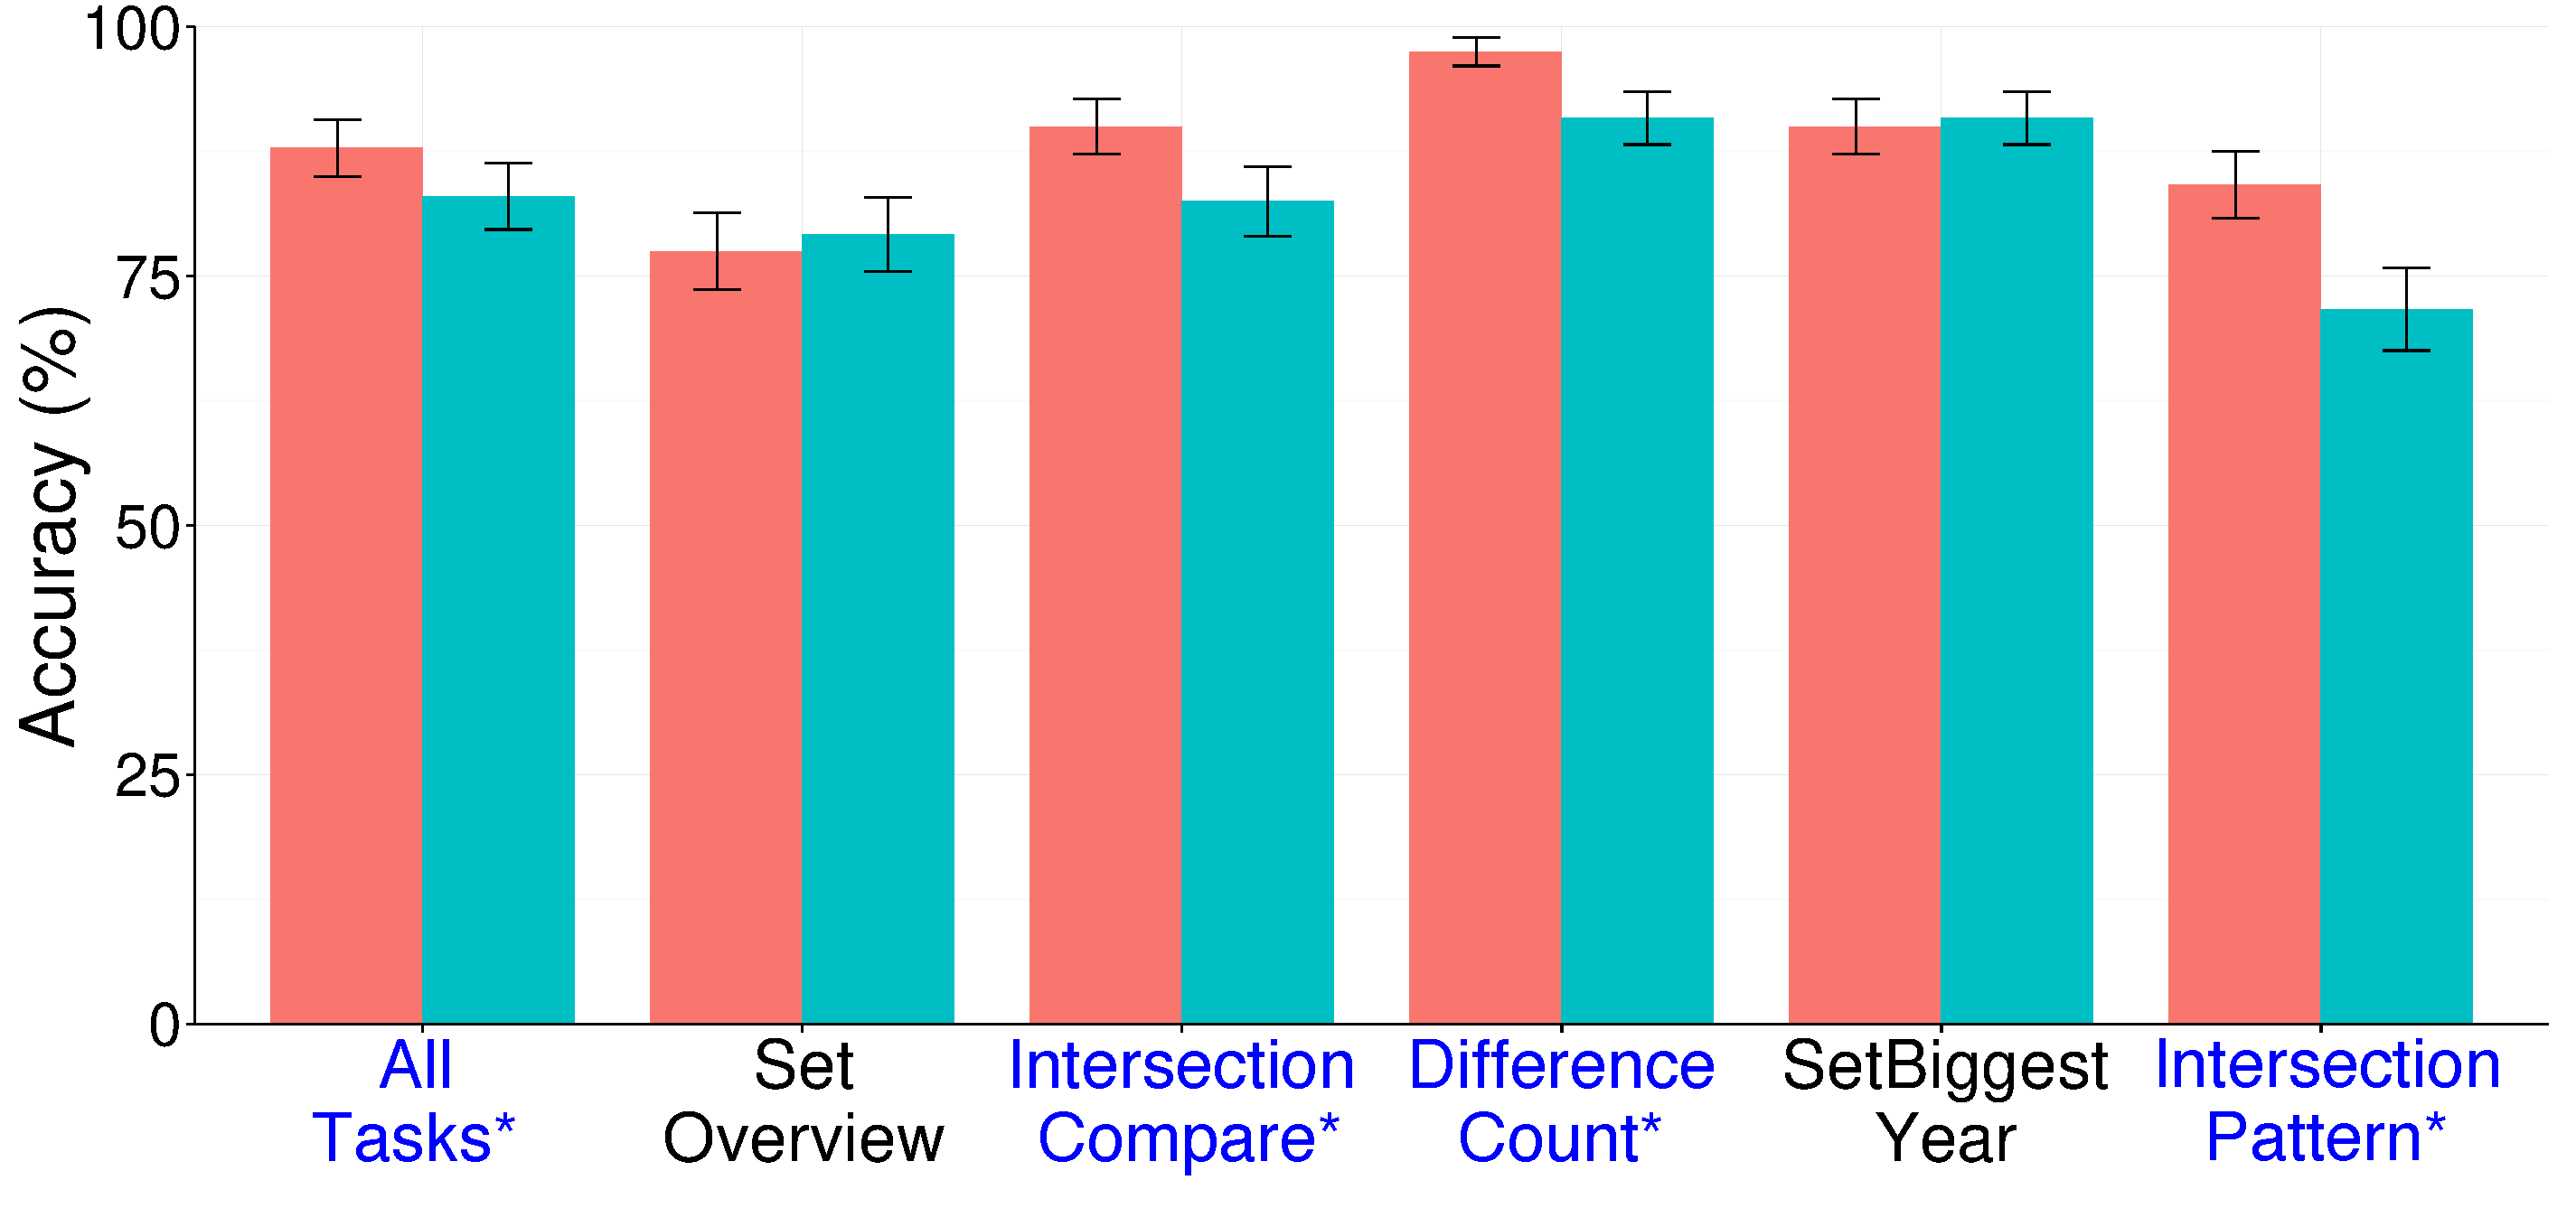
\includegraphics[width=.8\linewidth]{figure15b}}\\
	\subcaptionbox{Mean completion time (in seconds).\label{fig:time}}{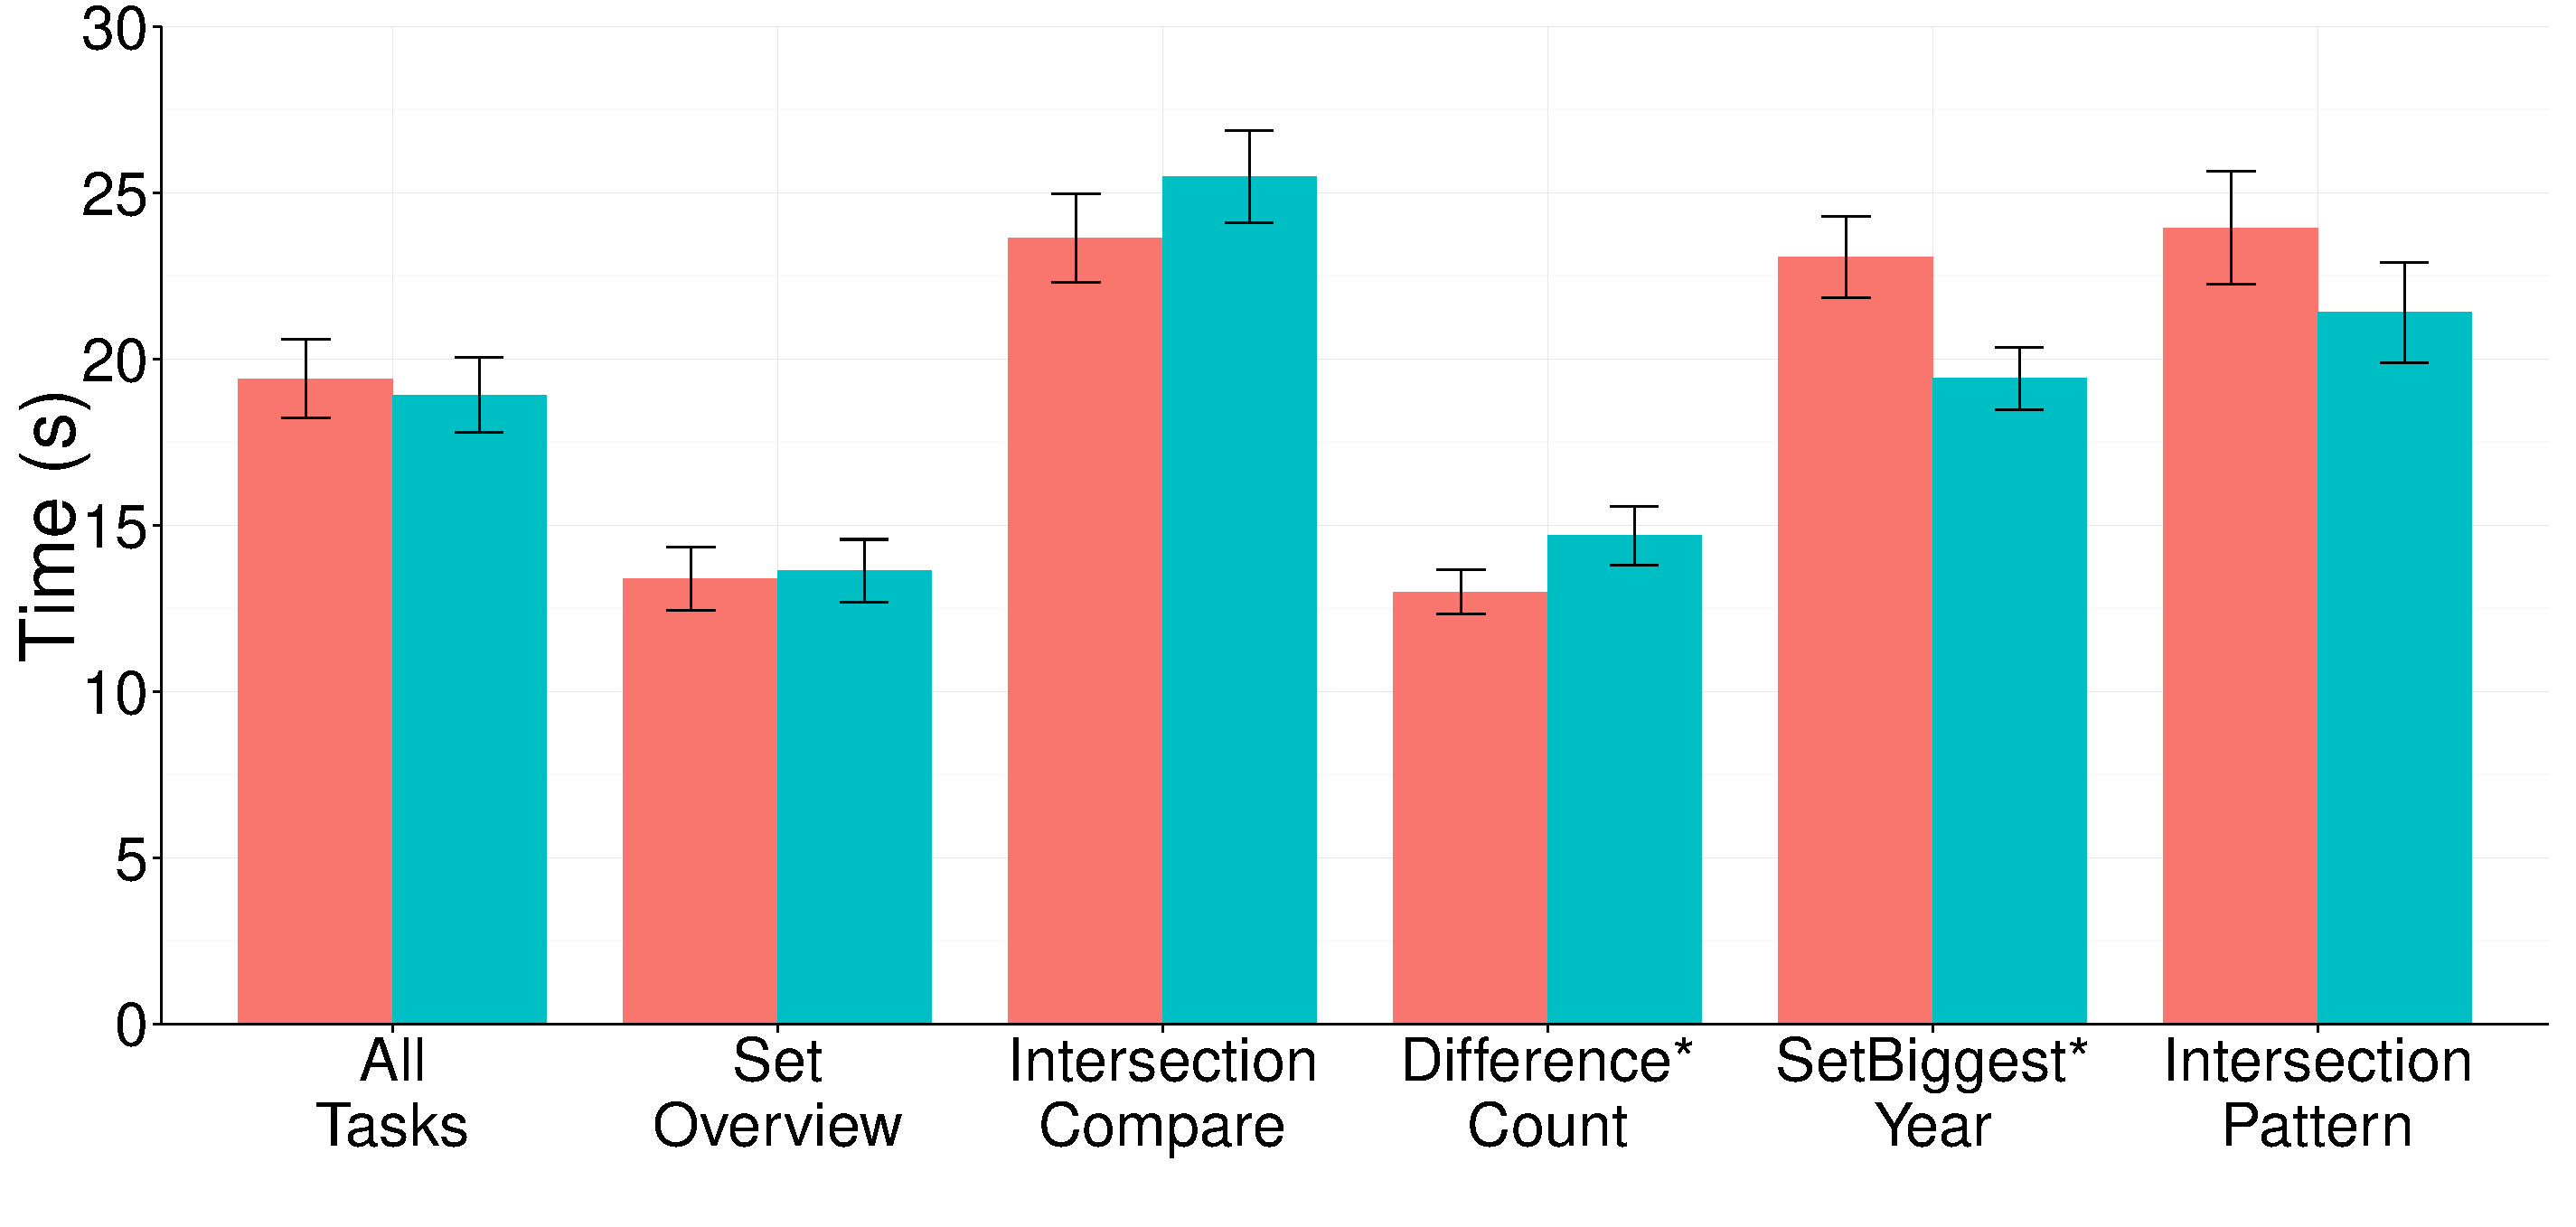
\includegraphics[width=.8\linewidth]{figure15c}}
	\caption[Mean accuracy and completion time for each task]{Mean accuracy and completion time for each task. Error bars show standard error. Tasks with significant effect are highlighted with a star (*).}
\end{figure}

\subsubsection{Time}
\autoref{fig:time} shows the mean completion time. The RM-ANOVA test revealed no significant main effect of visualization technique ($F(1,29)=.05, p=.82$), indicating that the completion time for TimeSets ($M=23.87,SD=9.18$) and KelpFusion ($M=23.72,SD=11.38$) were not significantly different. There was a significant main effect of task type ($F(4,116)=23.80, p<10^{-12}$). The visualization $\times$ task interaction was also significant ($F(4,116)=3.23,p<.05$), indicating that difference in completion time due to visualization technique was significantly different across tasks. To further investigate this, a paired t-test for each task was conducted. Significant effects were found in the DifferenceCount task ($p<.01$), indicating TimeSets is significantly faster in this task, and the SetBiggestYear task ($p<.01$), indicating KelpFusion is significantly faster in this task. Both tasks still had a significant effect with corrected p-value for multiple tests using Bonferroni correction.

\subsubsection{User Preference}
Participants were asked to rate both methods using a Likert scale from 1 (worst) to 5 (best) after they completed all the tasks. The following four questions were asked for each visualization technique:
\begin{itemize}
	\item How confident were the participants in answering the questions?
	\item How aesthetically pleasing were the visualizations?
	\item How cluttered were the visualizations?
	\item How strong was the sense of grouping?
\end{itemize}
\autoref{fig:ratings} shows the summary of user ratings. Fisher's exact tests found significant effects in all questions: Confidence ($p<.01$), Aesthetically Pleasing ($p<.01$), Not Cluttered ($p<.01$), and Sense of Grouping ($p<.0001$); indicating users preferred TimeSets to KelpFusion in those aspects.

\begin{figure}[p]
	\centering
	\subcaptionbox{How confident were they in answering the questions?} {
		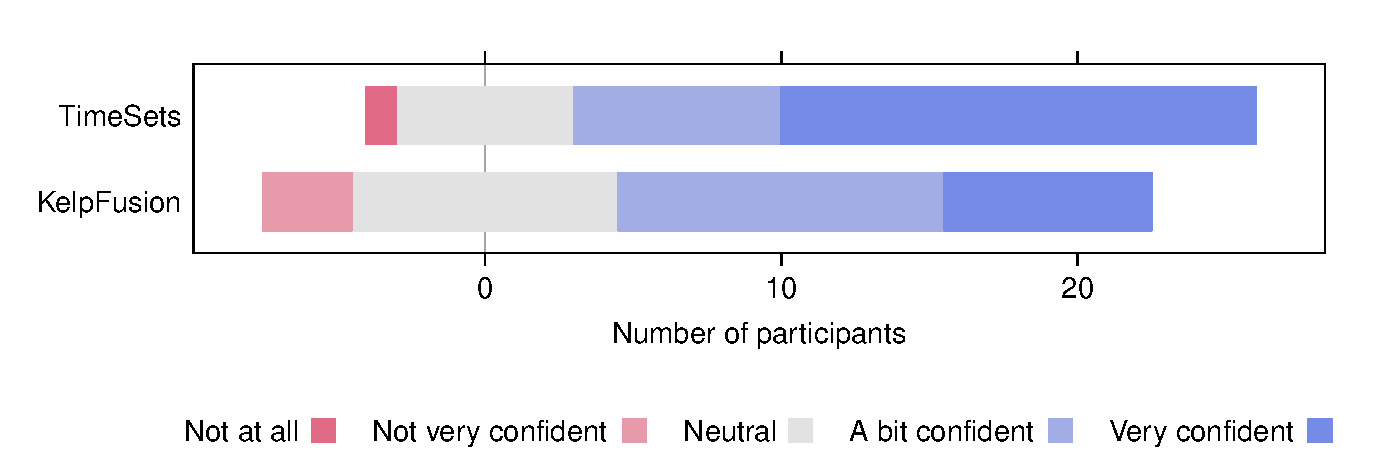
\includegraphics[width=.98\columnwidth]{figure16a}}
	\subcaptionbox{How aesthetically pleasing were the visualizations?}{
		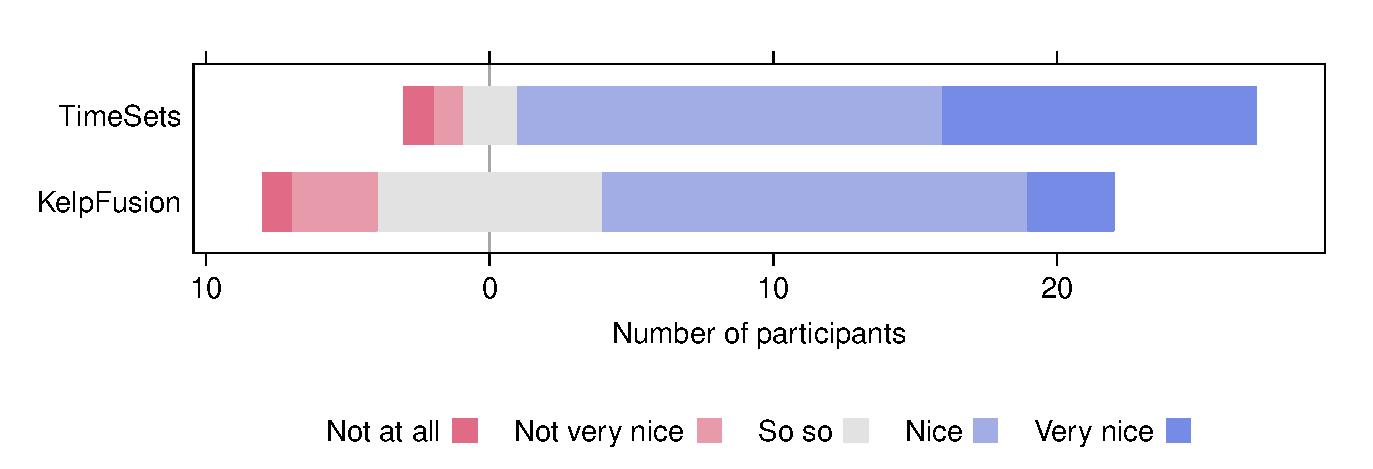
\includegraphics[width=.98\columnwidth]{figure16b}}
	\subcaptionbox{How cluttered were the visualizations?}{
		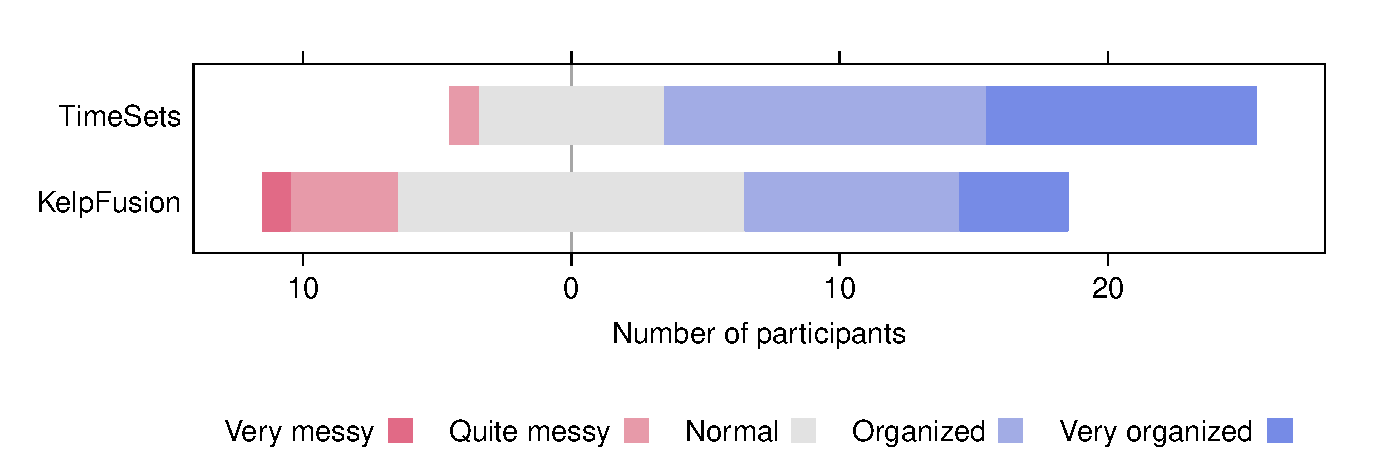
\includegraphics[width=.98\columnwidth]{figure16c}}
	\subcaptionbox{How strong was the sense of grouping?}{
		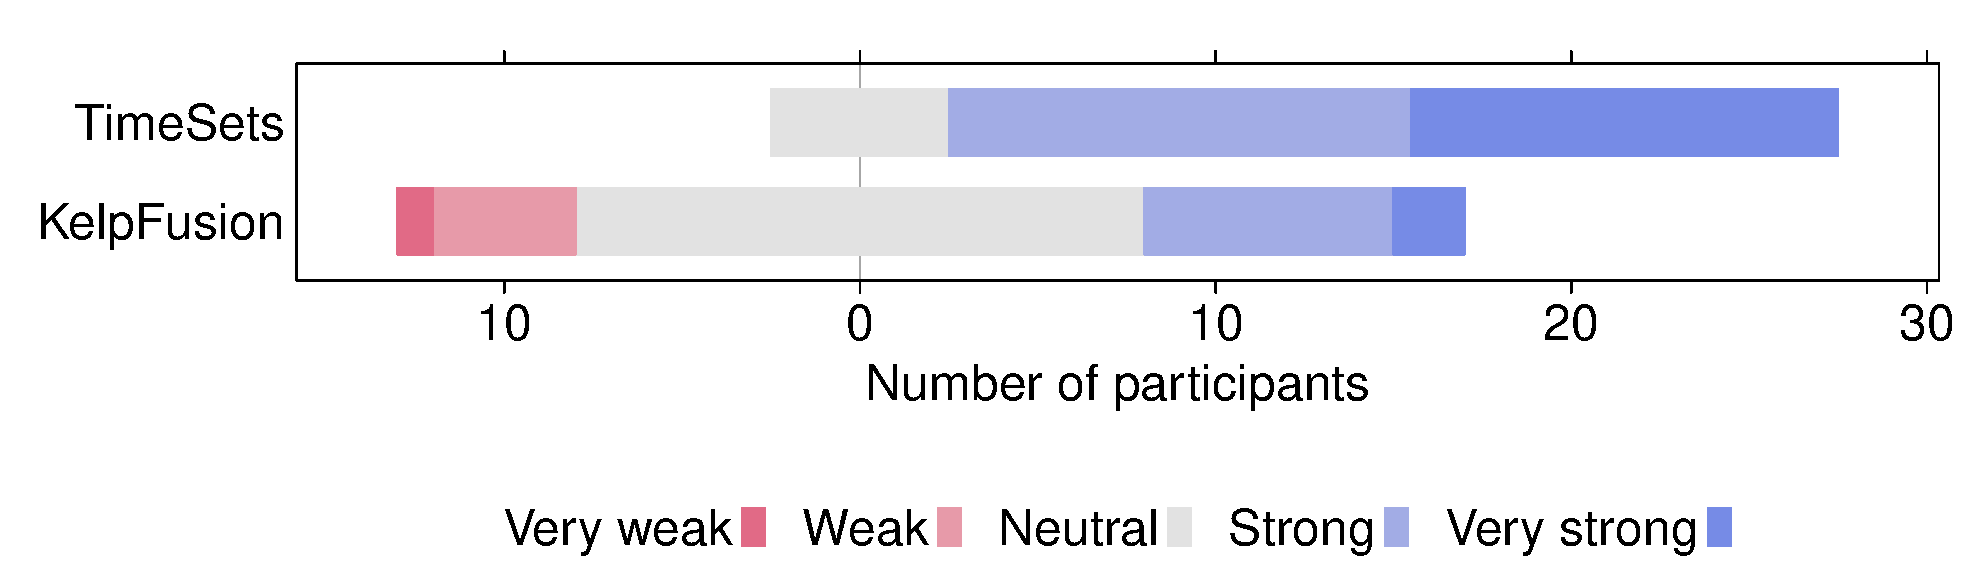
\includegraphics[width=.98\columnwidth]{figure16d}}
	\caption[Subjective user ratings of each technique for each question]{Subjective user ratings of each technique for each question. Bar width represents the number of participants selected the corresponding option.}
	\label{fig:ratings}
\end{figure}

\subsection{Discussion}
The results show that overall, TimeSets outperforms KelpFusion in accuracy, but not in completion time. This partly agrees with hypothesis \textbf{H1}.

For the \emph{SetOverview} task, there was no significant effect of visualization technique on either accuracy or completion time, which disagrees with hypothesis \textbf{H2}. The average accuracy of both methods is relatively low to other tasks in the experiment. Possible causes for TimeSets are discussed earlier in the hypothesis statement, and the edge length in KelpFusion -- a prominent visual feature -- is probably not a good size indicator either.

For intersection tasks, the results also show that TimeSets has higher accuracy than KelpFusion; however, their completion time performances are not significantly different. This partly confirms hypothesis \textbf{H3}. In TimeSets, shared events are highlighted by color gradient, thus participants are less likely to miscount them. In KelpFusion, shared events are horizontally aligned, because it shares the same layout as TimeSets. We observed that some participants tried to trace shared events using this way, which is prone to missing events, thus KelpFusion has similar speed but lower accuracy.

Hypothesis \textbf{H4}, about the DifferenceCount task, is supported by the results. Events that belong to a single set are clearly shown in TimeSets as a region with a single colored background. This helps improve performance in both accuracy and completion time.

The results show that KelpFusion has faster completion time than TimeSets for the SetBiggestYear task, but there is no significant difference in accuracy. This partly agrees with hypothesis \textbf{H5}. The vertical lines used to denote year boundaries in this task may have helped, by splitting the visual area into columns. To solve the task, participants count the number of events in each column and pick the highest one. A KelpFusion visualization is quite similar to a network, and edges connecting events within each column can make counting easier. This may explain why participants counted faster with KelpFusion, but had the same accuracy as with TimeSets.

To visualize sets, Bubble Sets~\cite{Collins2009a} uses a similar metaphor as TimeSets -- filling the area of same-set events with a unique color. However, KelpFusion outperforms Bubble Sets~\cite{Meulemans2013}, while TimeSets outperforms KelpFusion in solving similar tasks. One possible explanation is that the irregular shapes generated using iso-contours in Bubble Sets make set memberships difficult to perceive. Also, the layout in TimeSets groups same-set events together, which enables participants to easier count or estimate. Another reason could be that the color gradient in TimeSets may be more effective than color blending in Bubble Sets for visualizing shared events.

The participants preferred TimeSets in all four questions: confidence, aesthetics, readability, and sense of grouping. This supports hypotheses \textbf{H6}, \textbf{H7}, \textbf{H8} and \textbf{H9}. Half of the participants (15 out of 30) were more confident with TimeSets. Some of them commented that its set background made it easier to count events, especially for the intersections. Only four participants thought that they were more confident with KelpFusion (the other eleven thought they were at the same level of confidence). One said ``I can follow the links when counting, so I'm less likely to miss any''. Interestingly, three of these four participants actually had better accuracy with TimeSets. Half of the participants (15 out of 30) thought that TimeSets was more aesthetically pleasing than KelpFusion. Some of them said that they liked the curved boundaries and the smooth changing of colors. Only three participants favored KelpFusion. One of them commented that with TimeSets, his eyes were tired after looking at large areas with bright colors for a long time. More than half of the participants (17 out of 30) rated TimeSets as less cluttered than KelpFusion. One said ``TimeSets is more organized. I know event labels aren't important, but they seem easier to read.''. Three quarters of the participants (22 out of 30) agreed that TimeSets provided a stronger sense of grouping than KelpFusion. Many of them commented that KelpFusion figures looked more like a network than a group.